\begin{figure}[h]
    \centering
    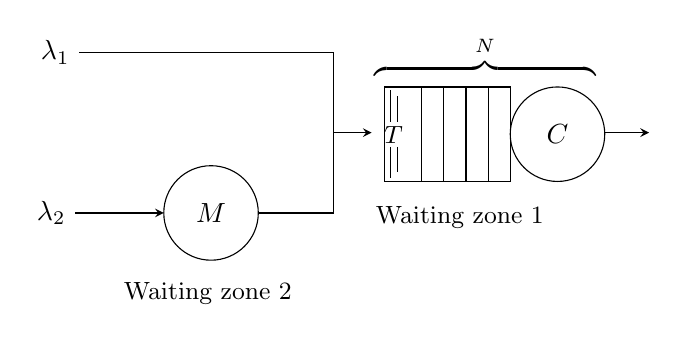
\begin{tikzpicture}[>=stealth, scale=0.8],

        % the circle in Queue 1
        \draw (2.25cm, -0.75cm) circle [radius=0.75cm] node {\(M\)};

        % The label below Queue 1 -> Waiting zone 2
        \node[anchor=north] at (2.2cm, -1.7cm) {\small{Waiting zone 2}};

        % the rectangle in Queue 2
        \draw (5, 1.25) -- ++(2cm, 0) -- ++(0, -1.5cm) -- ++(-2cm, 0);
        % the vertical lines in Queue 2
        \foreach \i in {1,...,4, 5.7}
        \draw (7cm-\i*10pt,1.25) -- +(0,-1.5cm);
        % The two vertical lines at the start of Queue 2
        \draw (7cm-54pt,1.2) -- +(0,-0.5cm);
        \draw (7cm-54pt,0.3) -- +(0,-0.5cm);
        \draw (7cm-51pt,1.1) -- +(0,-0.4cm);
        \draw (7cm-51pt,0.3) -- +(0,-0.4cm);

        % The label between the lines for T
        \node[anchor=north] at (5.15, 0.77 cm) {\small{\( T \)}};

        % The label above Queue 2 -> N
        \node[anchor=north] at (6.6cm, 2.2cm) {\(
            \overbrace{\qquad \qquad \qquad \qquad}^{N}
        \)};
        % The label below Queue 2 -> Waiting zone 1
        \node[anchor=north] at (6.2cm, -0.5cm) {\small{Waiting zone 1}};

        % the circle in Queue 2
        \draw (7.75,0.5) circle [radius=0.75cm] node {\(C\)};

        % Arrow line from Queue 2 outside
        \draw[->] (8.5,0.525) -- +(20pt,0);

        % Line from lambda_2 to Queue 1
        \draw[<-] (1.5,-0.75) -- +(-40pt,0) node[left] {\( \lambda_2 \)};
        % First line (horizontal) after Queue 1
        \draw[-] (3,-0.75) -- +(34pt,0);
        % Second line (vertical) after Queue 1
        \draw (4.2, 0.525) -- (4.2, -0.75);

        % First line (horizontal) from lambda_1
        \draw (4.2, 1.8) -- +(-115pt,0) node[left] {\( \lambda_1 \)};
        % Second line (vertical) from lambda_1
        \draw (4.2, 1.8) -- (4.2, 0.525);
        % Arrow line to Queue 2
        \draw[->] (4.2, 0.525) -- (4.8, 0.525);
    \end{tikzpicture}
    \caption{An equivalent model to the one described in
    Figure~\ref{fig:diagram_of_queueing_system}. The difference between the two
    diagrams is the formulation of waiting zone 2. The original diagram uses
    a node with no servers and a queueing capacity of \(M\) while this one uses
    \(M\) servers with no queueing capacity.}
    \label{fig:equivalent_diagram_of_queueing_system}
\end{figure}
